%
% -- Manlio Modugno

\documentclass{beamer} 
\usepackage{eulervm}
%\usepackage{booktabs}
\usepackage{listings}
\usepackage{bold-extra}
\usepackage{cancel}
\usepackage{fancybox}
\usepackage{soul}
\usepackage[english]{babel}
\usepackage[utf8]{inputenc}
\usepackage{hyperref}
\usepackage{amsmath}
%\hypersetup{colorlinks=true,urlcolor=blue}

\newcommand{\codefont}{\fontsize{6}{8}\selectfont}
\lstset{language=[Sharp]C, 
captionpos=b, 
frame=lines,
lineskip= 1pt, %space between lines
basicstyle=\codefont, 
keywordstyle=\color{blue}, 
commentstyle=\color{green}, 
stringstyle=\color{red}, 
numbers=left, 
numberstyle=\tiny, 
stepnumber=2,
numbersep=5pt,
breaklines=true, 
breakatwhitespace=false,
showstringspaces=false,
frame=single,
tabsize=2,
emph={double,bool,int,unsigned,char,true,false,void},
emphstyle=\color{blue},
emph={Assert,Test},
emphstyle=\color{red},
emph={[2]\using,\#define,\#ifdef,\#endif},
emphstyle={[2]\color{blue}}
}


\mode<presentation>
\definecolor{title_color}{RGB}{2,128,181} 
\usetheme{Ilmenau}
\usecolortheme[named=title_color]{structure}
\setbeamercolor{palette quaternary}{use=structure,fg=black,bg=white} %header footer color
\useoutertheme[subsection=false]{smoothbars}
\setbeamercovered{transparent}
\setbeamertemplate{navigation symbols}{}
\setbeamerfont{subsection in toc}{size=\scriptsize}

\title{The Interface Segregation Principle}
\author{Manlio Modugno}
\institute[GMTechnologies] 

\date[]{The Interface Segregation Principle}

\subject{}

\graphicspath{{img/}}
\pgfdeclareimage[height=0.6cm]{mfg-logo}{img/mfgLogo}
\logo{\pgfuseimage{mfg-logo}}

%
% Content start
%
\begin{document}
\begin{frame}
  \titlepage
\end{frame}

\begin{frame}
  \frametitle{Topics}
  \tableofcontents
\end{frame}


\section{Intro}
\subsection{Intro}
\begin{frame}
  \frametitle{Intro}
  \begin{itemize}
	\item<+-> Deals with fat (i.e. not cohesive) interfaces.
	\item<+-> Different clients use different group of methods 
	\item<+-> Clients should only know about abstract base classes that have cohesive interfaces 
	\item<+-> def: \textbf{Clients should not be forced to depend on methods they do not use.}
   \end{itemize}
\end{frame}

\section{Interface Pollution}
\subsection{Interface Pollution}
\begin{frame}[containsverbatim]
	\frametitle{Interface Pollution}
	Consider a security system where \textit{Door} objects can be un/locked and know whether they are open or closed\\
	\begin{lstlisting}
interface Door {
	Lock();
	Unlock();
	IsDoorOpen();
}
	\end{lstlisting}
\textit{TimedDoor} is an implementation that needs to sound an alarm when door has been left open and works with \textit{Timer}\\
	\begin{lstlisting}
public class Timer{
	void Register(int timeout, TimerClient client) {/*code*/}
}
public interface TimerClient{
	void timeOut();
}
	\end{lstlisting}
\end{frame}

\begin{frame}
  \frametitle{Interface Pollution}
  \begin{itemize}
	\item<+-> An object subscribe to timeout notification calling \textit{Register} function 
	\item<+-> \textit{timeout} method is invoked when timeout expires 
	\item<+-> How can \textit{TimerClient} communicate back to \textit{TimeDoor} expiration time?
   \end{itemize}
\end{frame}

\begin{frame}
	\frametitle{Interface Pollution}
	Force \textit{Door} to inherit from \textit{TimerClient}
	\begin{center}
	\fbox{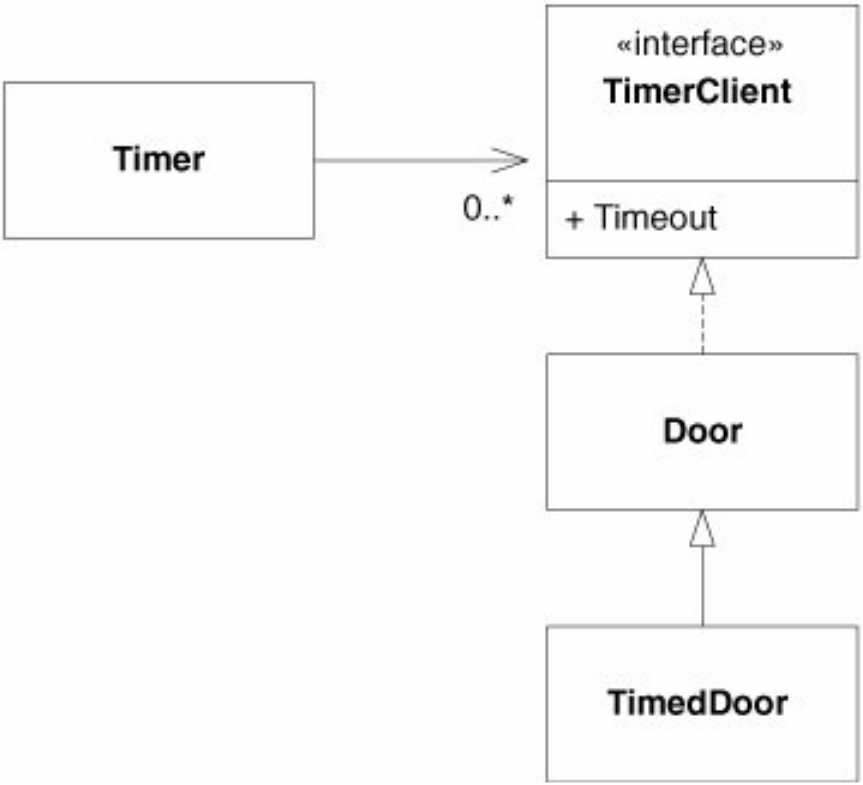
\includegraphics[scale=0.3]{ispBad}}
	\end{center}
\end{frame}

\begin{frame}
  \frametitle{Interface Pollution}
  \begin{itemize}
	\item<+-> \textit{Door} depends on \textit{TimerClient}.. not all \textit{Door}s need this kind of coupling... 
	\item<+-> ..we could have degenerate solutions violating LSP..\\
	\item<+-> Interface is polluted with a method that does not require.. introduced to satisfy a particular need..
   \end{itemize}
\end{frame}

\section{Separate Clients Mean Separate Interfaces}
\subsection{Separate Clients Mean Separate Interfaces}
\begin{frame}
  \frametitle{Separate Clients Mean Separate Interfaces}
  \begin{itemize}
	\item<+-> \textit{Door} and \textit{TimerClient} represent interfaces that are used by completely different clients.. they should use different interfaces 
	\item<+-> Usually a change in interface implies a change in clients..
	\item<+-> But the other way around is also possible.. a client \textit{forces} a change in the interface..
	\item<+-> When client are forced to depend on methods don't use, are subject to changes of those methods..
	\item<+-> ..a coupling problem arise
   \end{itemize}
\end{frame}

\section{Class Interfaces versus Object Interfaces}
\subsection{Class Interfaces versus Object Interfaces}
\begin{frame}[containsverbatim]
	\frametitle{Class Interfaces versus Object Interfaces}
  \begin{itemize}
	\item<+-> \textit{TimedDoor} has two interfaces used by separate clients: \textit{Timer} and users of \textit{Door}..
	\item<+-> Those must be implemented in the same object, since implementations manipulate same data..
	\item<+-> But how to do it respecting ISP?.. How to separate interfaces when they must remain together?
	\item<+-> Answer is that client don't need to access an object through an interface; they can access it through delegation or through a base class.
   \end{itemize}
\end{frame}

\subsection{Separation Through Delegation}
\begin{frame}
  Define an object that derives from \textit{TimerClient} and delegates to \textit{TimedDoor} \\
  \frametitle{Separation Through Delegation}
  \begin{center}
	\fbox{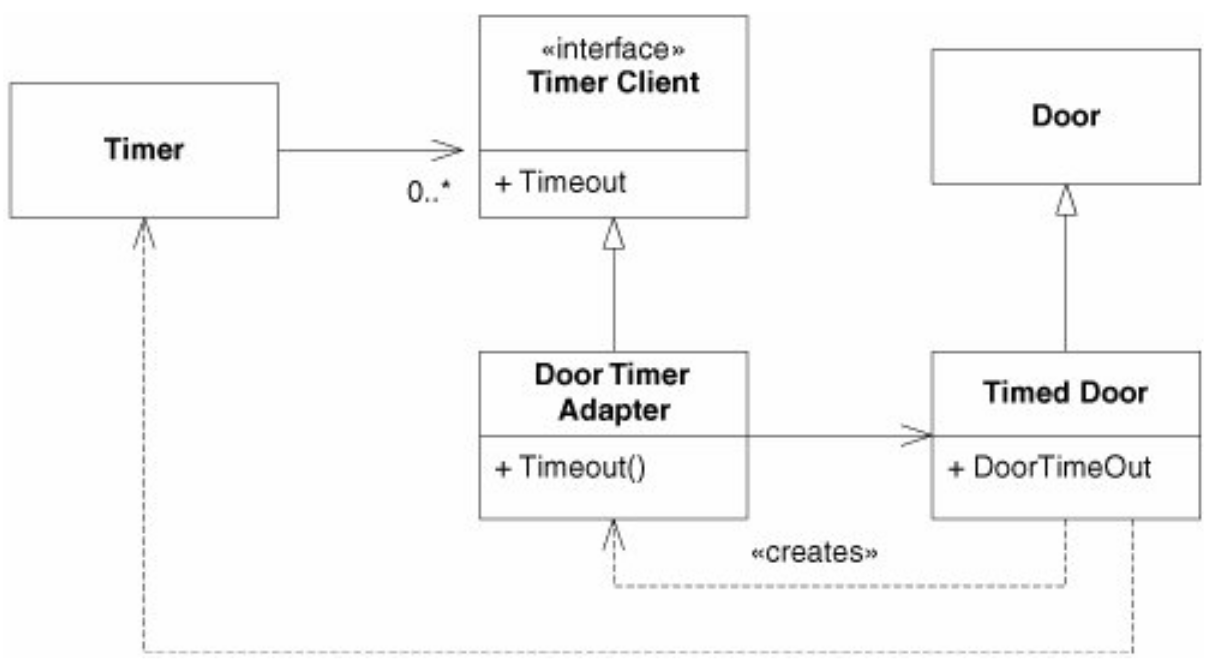
\includegraphics[scale=0.2]{doorTimeAdapter}}
	\end{center}
\end{frame}

\begin{frame}
  \frametitle{Separation Through Delegation}
  \begin{itemize}
	\item<+-> When a timer registration is needed; \textit{TimedDoor} creates a \textit{DoorTimerAdapter}
	\item<+-> When the \textit{Timer} sends the \textit{TimeOut} message to the \textit{DoorTimerAdapter} , the \textit{DoorTimerAdapter} delegates the message back to the \textit{TimedDoor}
	\item<+-> This solution is ISP compliant, prevents coupling of \textit{Door} clients to \textit{Timer}
	\item<+-> Is a general purpose solution but has a little overhead...
   \end{itemize}
\end{frame}

\subsection{Separation Through Multiple Inheritance}
\begin{frame}
  \frametitle{Separation Through Delegation}
  \textit{TimedDoor} inherits from both \textit{Door} and \textit{TimerClient} \\
  Clients use same objects through separate interfaces \\
  \begin{center}
	\fbox{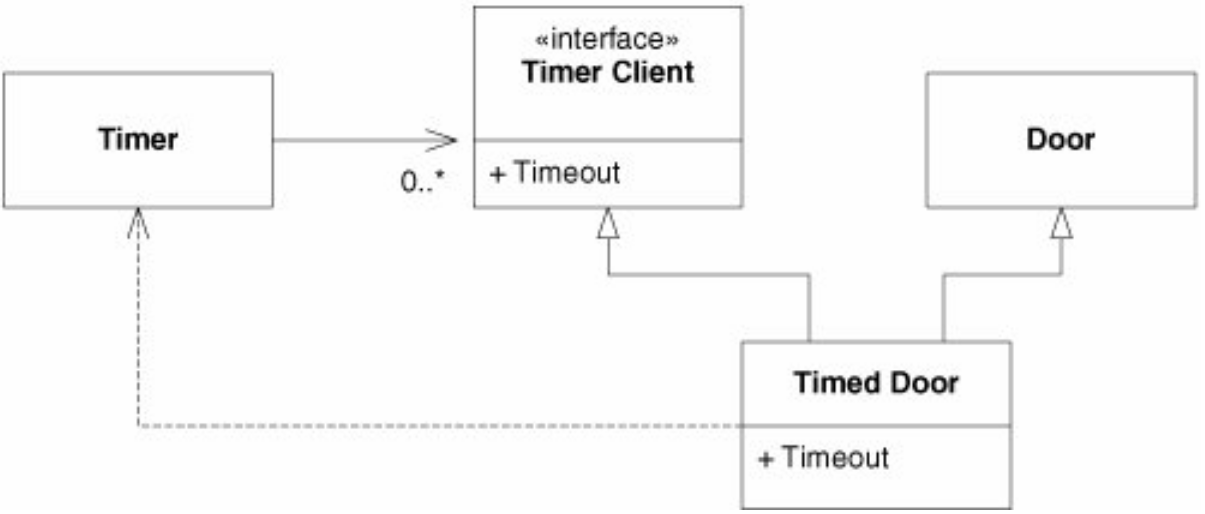
\includegraphics[scale=0.2]{multiIhn}}
  \end{center}
\end{frame}

\section{The ATM User Interface Example}
\subsection{The ATM User Interface Example}
\begin{frame}
  \frametitle{The ATM User Interface Example}
  ATM needs to be very flexible: output may be translated, showed on screen, braille or spoken.. \\
  \begin{center}
	\fbox{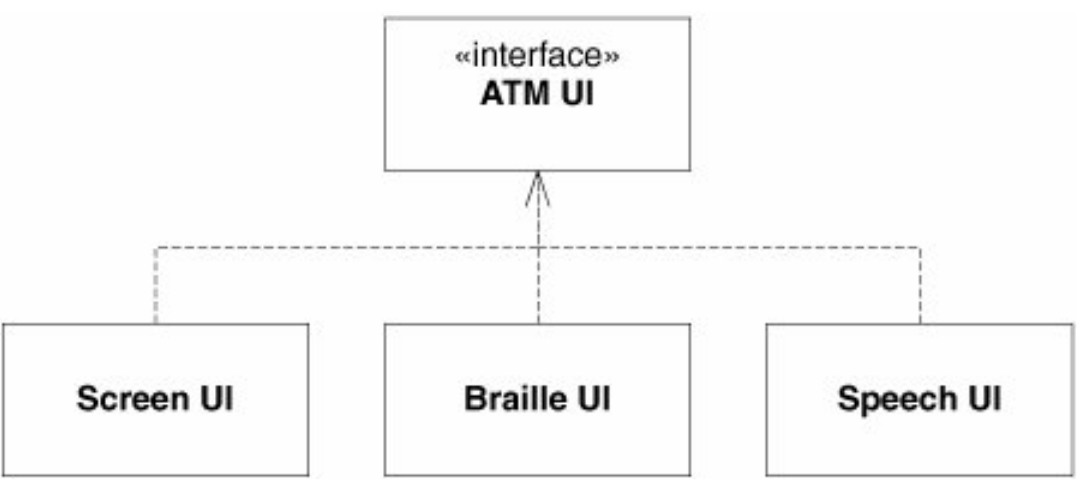
\includegraphics[scale=0.2]{atm}}
  \end{center}
\end{frame}

\begin{frame}
  \frametitle{The ATM User Interface Example}
  Moreover exist derived transaction that interact with UI.. \\
  \begin{center}
	\fbox{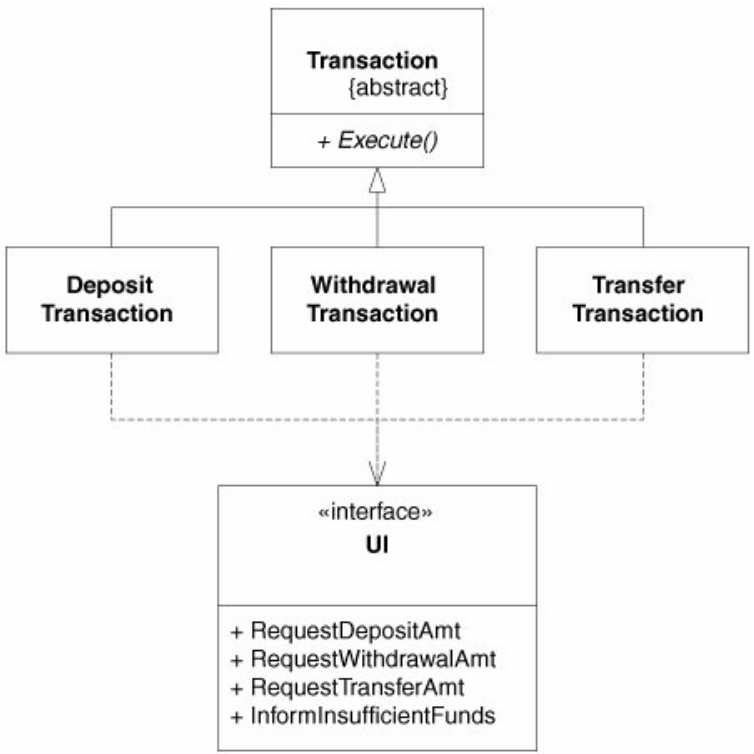
\includegraphics[scale=0.2]{transaction}}
  \end{center}
\end{frame}


\begin{frame}
  \frametitle{Separation Through Delegation}
  \begin{itemize}
	\item<+-> Each transaction is using UI methods that no other class uses..
	\item<+-> A change occuring in a derivative can force a change in UI affecting all the other derivatives or any other UI dependent..
	\item<+-> Supposing an add of a new transaction... we need to add a method to UI also.. this implies a rebuilt of dependent of UI..
	\item<+-> Segregating UI interface into individual interfaces avoids useless coupling...
   \end{itemize}
\end{frame}


\begin{frame}[containsverbatim]
	\frametitle{LSP violation}
	But if in the code already exists a function like: \\
	\begin{lstlisting}
void g(Rectangle r){
  r.Width = 5;
  r.Height = 4;
  if(r.Area() != 20)
    throw new Exception("Bad area!");
}
	\end{lstlisting}
	we have a problem... \\
\end{frame}

\begin{frame}
  \frametitle{LSP violation of g function}
  \begin{itemize}
	\item<+-> Author of g assumed that changing the width of a Rectangle leaves its height unchanged (and this is reasonable!)
	\item<+-> g is fragile with respect to Square / Rectangle hierarchy.. because a \textit{Square} \textbf{it's not} a \textit{Rectangle}! (in this context)
	\item<+-> One might argue that developer of g function had no right to make assumption of independent measure between height and width...
	\item<+-> but here, real error is the hierarchy created by second developer that broke an invariant of \textit{Rectangle} inserting a \textit{Square}!
   \end{itemize}
\end{frame}

\subsection{Validity is not intrinsic}
\begin{frame}
  \frametitle{Validity is not intrinsic}
  \begin{itemize}
	\item<+-> LSP leads to an important conclusion: ``A model, viewed in isolation, cannot be meaningfully validated''
	\item<+-> ..the validity of a model can be expressed only in terms of
its clients.. in fact \textit{Rectangle} and \textit{Square} taken in isolation were valid..
	\item<+-> ..but when used from a client model broke down...
	\item<+-> When considering whether a particular design is appropriate, one cannot simply view the solution in isolation.
	\item<+-> \textbf{One must view it in terms of the reasonable assumptions made by the users of that
design} (...pay attention to needless complexity!)
   \end{itemize}
\end{frame}

\subsection{ISA is about behavior}
\begin{frame}
  \frametitle{ISA is about behavior}
  \begin{itemize}
	\item<+-> Why something went wrong with Rectangle/Square relationship..? 
	\item<+-> isn't a Square a Rectangle ..? Isn't so natural..?
	\item<+-> maybe for everyone except that for g's author...
	\item<+-> \textbf{Behavior} of \textit{Square} is not consistent with g's expectation.. 
	\item<+-> \textbf{Behaviorally a Square is not a Rectangle!}.. and it is behavior that software is really all about
	\item<+-> LSP make a strict definition for subtype relationship
   \end{itemize}
\end{frame}

\subsection{Design by contract}
\begin{frame}
  \frametitle{Design by contract}
  \begin{itemize}
	\item<+-> How to know what clients behaviorally expect?
	\item<+-> Using DBC, the author of a class explicitly states the contract for that class.
	\item<+-> ..could be tricky.. writing test It's better..
   \end{itemize}
\end{frame}

\section{A Real-World Example}
\subsection{Motivation}
\begin{frame}
  \frametitle{A Real-World Example}
  \begin{itemize}
	\item<+-> Author purchased a third-party lib that managed \textit{Bag}s and \textit{Set}s data structure..
	\item<+-> Exist two variety \textit{bounded}, based on array, and \textit{unbounded}, based on linked list
	\item<+-> \textit{BoundedSet} specify by constructor max size of elements...
	\item<+-> \textit{UnoundedSet} has not limit in size allocation..
	\item<+-> To avoid coupling author wrapped libraries in his own interfaces
   \end{itemize}
\end{frame}

\subsection{wrapping}
\begin{frame}
  \frametitle{A Real-World Example}
  \fbox{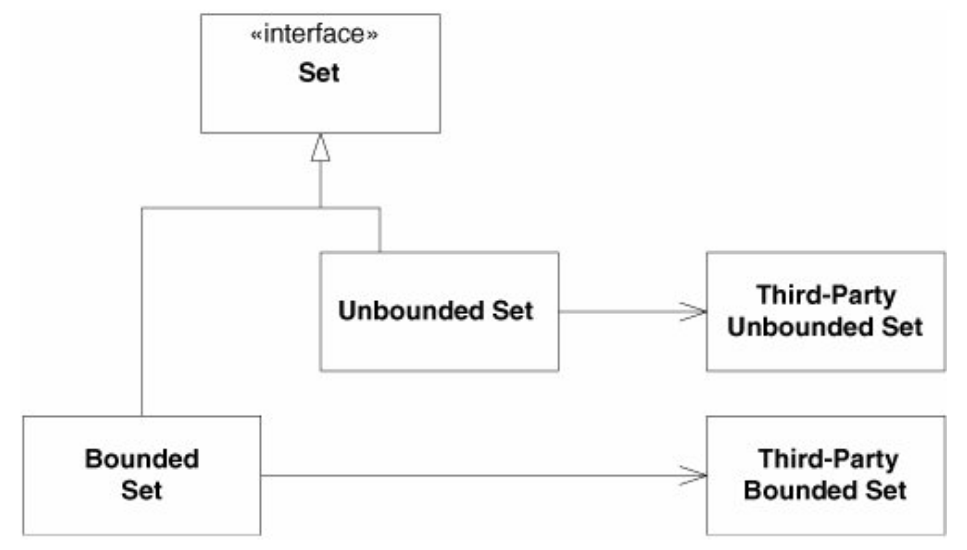
\includegraphics[scale=0.3]{wrap}}
\end{frame}

\begin{frame}[containsverbatim]
	\frametitle{A Real-World Example}
	Interface \textit{Set} to unify unbounded and bounded variety\\
	\begin{lstlisting}
	public interface Set{
      void Add(object o);
      void Delete(object o);
      bool IsMember(object o);
	}
    ...
    void PrintSet(Set s){
	  foreach(object o in s)
  	  Console.WriteLine(o.ToString());
	}	
	\end{lstlisting}
\end{frame}

\begin{frame}
  \frametitle{A Real-World Example}
  \begin{itemize}
	\item<+-> It's nice to don't care about what kind of Set to use... 
	\item<+-> It's up to programmer to choose which kind to use.. for memory / speed issues..
	\item<+-> ...
   \end{itemize}
\end{frame}

\subsection{problem}
\begin{frame}
  \frametitle{Problem}
	Author added a \textit{PersistentSet} that can be stored and retrieved..The third-party version defined accept only \textit{PersistentObject} \\
	\begin{center}
	\fbox{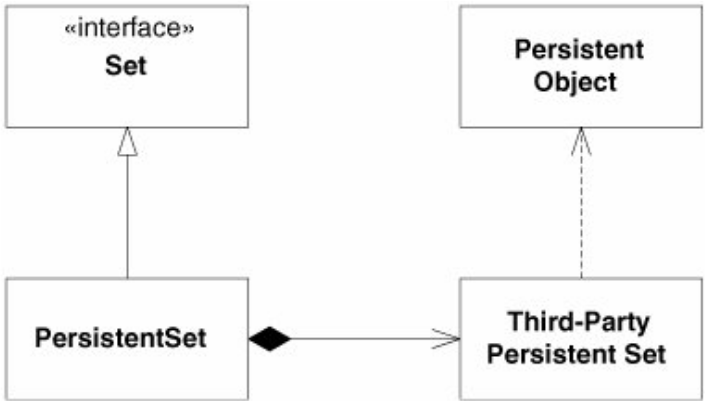
\includegraphics[scale=0.3]{persistent}}
	\end{center}
\end{frame}

\begin{frame}[containsverbatim]
  \frametitle{Problem}
  \begin{itemize}
	\item When a client is adding members to the base class Set, that client cannot be sure whether the Set might be a PersistentSet 
	\item ... so It can't know whether the elements it adds should be derived from \textit{PersistentObject}
	\item code like PersistentSet\#Add introduce potential runtime problems..
	\item Existing functions that used \textit{Set} as reference in signature can now broke down because of \textit{PersistentSet}
   \end{itemize}
   \begin{lstlisting}
//PersistentSet#Add
   
void Add(object o){
  PersistentObject p = (PersistentObject)o;
  thirdPartyPersistentSet.Add(p);
}
	\end{lstlisting}
\end{frame}

\subsection{First solution, not conforming to LSP}
\begin{frame}
  \frametitle{First solution, not conforming to LSP}
	\begin{itemize}
	\item<+-> A first approach was by convention..   
	\item<+-> ...it's a powerful principle.. but can have drawbacks..
	\item<+-> an unfocused developer can violate conventions...
	\item<+-> ...we should share conventions and than change them if necessary..
   \end{itemize}
\end{frame}

\subsection{An LSP-compliant solution}
\begin{frame}
  \frametitle{An LSP-compliant solution}
	\begin{itemize}
	\item<+-> \textit{PersistentSet} is not a subtype of \textit{Set} yet they share some feature...
	\item<+-> ...it's only the \textit{add} method that cause problem with LSP
   \end{itemize}
\end{frame}

\begin{frame}
  \frametitle{An LSP-compliant solution}
	A new interface is defined with common features \\
	\begin{center}
	\fbox{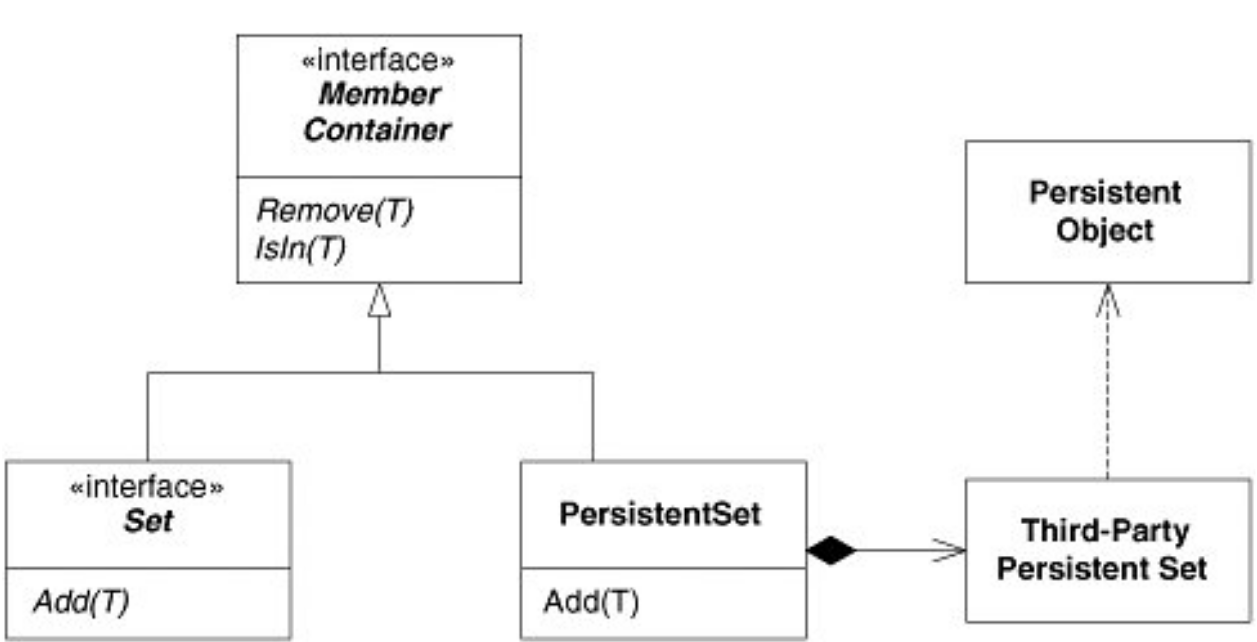
\includegraphics[scale=0.22]{lspGood}}
	\end{center}
\end{frame}

\section{Factoring Instead of Deriving}
\subsection{Factoring Instead of Deriving}
\begin{frame}[containsverbatim]
	\frametitle{Factoring Instead of Deriving}
	At first, these two classes appear to be \textbf{natural} candidates for inheritance. \textit{LineSegment} needs every member variable and every member function declared in \textit{Line} and override \textit{isOn}\\
	\begin{lstlisting}
public class Line{
  private Point p1;
  private Point p2;
  public Line(Point p1, Point p2){this.p1=p1; this.p2=p2;}
  public Point P1 { get { return p1; } }
  public Point P2 { get { return p2; } }
  public double Slope { get {/*code*/} }
  public double YIntercept { get {/*code*/} }
  public virtual bool IsOn(Point p) {/*code*/}
}
public class LineSegment : Line{
  public LineSegment(Point p1, Point p2) : base(p1, p2) {}
  public double Length() { get {/*code*/} }
  public override bool IsOn(Point p) {/*code*/}
}
	\end{lstlisting}
\end{frame}

\begin{frame}
  \frametitle{Factoring Instead of Deriving}
	\begin{itemize}
	\item<+-> A user of \textit{Line} in a plane (as function!) has the right to expect that isOn(YIntercept) is always true...
	\item<+-> .. but for a \textit{Segment} this is not always true!
	\item<+-> depending on context, a compromise can be \textbf{profitable} than perfection.. 
	\item<+-> However, conformance to LSP should not be surrendered lightly..
   \end{itemize}
\end{frame}

\begin{frame}[containsverbatim]
	\frametitle{Factoring Instead of Deriving}
	\textit{LinearObject}factors out the common functionalities excluding \textit{IsOn} method. Users of \textit{Line} are safe and assumption od \textit{isOn} cannot be made\\
	\begin{lstlisting}
public abstract class LinearObject{
  private Point p1;
  private Point p2;
  public LinearObject(Point p1, Point p2)  {this.p1=p1; this.p2=p2;}
  public Point P1 { get { return p1; } }
  public Point P2 { get { return p2; } }
  public double Slope { get {/*code*/} }
  public double YIntercept { get {/*code*/} }
  public virtual bool IsOn(Point p) {/*code*/}
}
public class Line : LinearObject{
  public Line(Point p1, Point p2) : base(p1, p2) {}
  public override bool IsOn(Point p) {/*code*/}
}
public class LineSegment : LinearObject{
  public LineSegment(Point p1, Point p2) : base(p1, p2) {}
  public double GetLength() {/*code*/}
  public override bool IsOn(Point p) {/*code*/}
}
	\end{lstlisting}
\end{frame}


\section{Heuristics and Conventions}
\subsection{Heuristics and Conventions}
\begin{frame}
  \frametitle{How to smell LSP violations?}
  \begin{itemize}
	\item<+-> Derivative classes somehow remove functionality from their base classes..
	\item<+-> A derivative that does less than its base is usually not substitutable for that base and therefore violates LSP
	\item<+-> degenerate function (i.e. empty function) can be indicative of LSP violation
   \end{itemize}
\end{frame}

\section{Conclusion}
\subsection{Conclusion}
\begin{frame}
  \frametitle{Conclusion}
  \begin{itemize}
	\item<+-> OCP keep applications maintainable, reusable and robust..
	\item<+-> LSP is one of the prime enablers of OCP.. because substitutability of subtypes allows a
module, expressed in terms of a base type, to be extensible without modification
	\item<+-> The term IS-A is too broad to act as a definition of a subtype. The true definition of a subtype is substitutable, where substitutability is defined by either an explicit or implicit contract.
   \end{itemize}
\end{frame}

\end{document}
